\newpage
\phantomsection
\chapter{Desarrollo}

\phantomsection
\section{Definición de identidad de marca}

    \phantomsection
    \subsection{Presentación de identidad corporativa: KERALYTIX}

        En el marco del desarrollo del producto, se definió la marca KERALYTIX como identidad corporativa del proyecto. El isotipo que la acompaña se muestra en la Figura~\ref{fig:logo_keralytix}.

        \begin{figure}[H]
            \centering
            
\includegraphics[width=0.45\textwidth]{img/logo_keralytix.png}
            \caption{Logotipo de la marca KERALYTIX.}
            \label{fig:logo_keralytix}
        \end{figure}

    \phantomsection
    \subsection{El nombre: composición y motivación}

        El nombre KERALYTIX es un neologismo creado a partir de la fusión de dos raíces. Por un lado, ``Kera-'', tomada del griego \textit{keras} (cuerno), que en la terminología médica dio origen al prefijo \textit{querato-}, referido a la córnea, y que delimita el campo de acción anatómico y clínico del producto. Por otro, el sufijo ``-lytix'', derivado del inglés \textit{analytics}, que expone el motor tecnológico del proyecto: el análisis de datos.

    \phantomsection
    \subsection{El logotipo (isotipo)}

        El logotipo (Figura~\ref{fig:logo_keralytix}) fue diseñado para abstraer la dualidad del producto (medicina y tecnología), alejándose de los clichés visuales médicos (como la silueta de un ojo con pestañas) para enfocarse en la precisión de los datos.

        \begin{itemize}[leftmargin=*]
            \item \textbf{Topografía y ectasia:} La estructura base está formada por curvas de nivel, que evocan los mapas de elevación anterior y posterior obtenidos con los equipos de topografía corneal. La deformación asimétrica que rompe la esfericidad de los anillos hacia un vértice inferior representa visualmente la patología: el queratocono.

            \item \textbf{Red neuronal y detección de anomalías:} Los puntos sólidos negros distribuidos sobre las curvas representan los nodos de una red neuronal, es decir, el modelo de IA que analiza los mapas corneales.

            \item \textbf{Estética monocromática:} El uso de líneas continuas en negro sólido asegura que el símbolo mantenga su legibilidad tanto en la interfaz oscura (\textit{dark mode}) del \textit{software} como en los informes impresos que recibirá el especialista.
        \end{itemize}

    \phantomsection
    \subsection{Identidad de marca y posicionamiento}

        \begin{itemize}[leftmargin=*]
            \item \textbf{Propuesta de valor (\textit{tagline}):} La bajada ``DIAGNÓSTICO DE QUERATOCONO IMPULSADO POR IA'' en un solo renglón ancla la abstracción del logo. Actúa como una declaración funcional que no deja margen a interpretaciones erróneas, un requisito clave en la comunicación de productos médicos.

            \item \textbf{Posicionamiento:} La identidad visual define a KERALYTIX como una herramienta de grado médico: aséptica, rigurosa y tecnológica.

            \item \textbf{Perfil de mercado:} La marca está pensada para un entorno B2B\footnote{Por sus siglas en inglés, \textit{Business to Business}: venta de productos o servicios entre empresas u organizaciones.}. Su estética busca inspirar la confianza y previsibilidad que exige el responsable de un hospital o de un sistema de salud pública al adquirir tecnología, al mismo tiempo que ofrece el atractivo moderno que busca el oftalmólogo independiente en su consultorio privado.
        \end{itemize}

\phantomsection
\section{Relevamiento clínico y análisis exploratorio de datos (EDA)}

    Tal como se planteó en la primera fase de la propuesta metodológica, se estableció contacto con diferentes centros de salud y profesionales del área de oftalmología, con el fin de reunir muestras locales anonimizadas que permitan evaluar el modelo con datos de la región. Las solicitudes se encuentran en curso y, hasta que se concreten, el trabajo continúa sobre los datos públicos del \textit{dataset} CornOrb, disponible en Zenodo~\cite{zenodo}.

    \phantomsection
    \subsection{Centros de salud y profesionales contactados}

        Los centros de salud y profesionales contactados hasta la fecha se detallan en la Tabla~\ref{tabla:centros_contactados}. Además de centros de Misiones, se incluyeron instituciones de otras provincias y del exterior, con el objetivo de ampliar las posibilidades de obtener muestras.

        \begingroup \setstretch{1.1}
        \begin{longtblr}[
            caption = Centros de salud y profesionales de oftalmología contactados,
            label = tabla:centros_contactados
            ]{
                colspec = {X[l,m] Q[l,m,4cm]},
                cells = {font=\small},
                row{1} = {bg=gray!15, font=\small\bfseries, halign=c},
                hlines, vlines,
                rowsep = 3pt, colsep = 5pt
            }

            Centro de salud o profesional & Ubicación \\

            Centro de Ojos Misiones Alta Complejidad & Posadas \\

            Clínica de Ojos Cáceres Zorrilla & Posadas \\

            Clínica de Ojos Maldonado Bas & Córdoba \\

            Universidad Hospital Italiano & Buenos Aires \\

            Dr. Óscar Mallo & Buenos Aires \\

            Clínica de Ojos Córdoba & Córdoba \\

            Clínica de Ojos Dr. Nano & Buenos Aires \\

            Clínica Vidavas & Perú \\

            Clínica de Ojos Dr. Santiago Barreyro & Posadas \\

        \end{longtblr}
        \endgroup

        Estos contactos constituyen el punto de partida para conformar el lote de muestras locales anonimizadas previsto en la propuesta metodológica. Si las muestras se obtienen durante el PFI, se utilizarán para una primera evaluación del modelo con datos de la región; su uso para una validación clínica formal corresponde a la proyección del producto (ver sección Alcance y limitaciones).

    \phantomsection
    \subsection{Conjunto de datos de trabajo}

        Mientras se concretan las solicitudes de muestras locales, el análisis se realiza sobre el \textit{dataset} CornOrb~\cite{zenodo}. Este recurso reúne 1.454 registros correspondientes a ojos de 744 pacientes, estudiados con un equipo Orbscan~3 en centros de oftalmología de Argelia. Para cada ojo se proporcionan cuatro mapas corneales (axial, anterior, posterior y paquimetría) en formato de imagen, junto con un archivo de datos clínicos que incluye la etiqueta diagnóstica: normal o queratocono. Según la documentación del \textit{dataset}, las etiquetas fueron asignadas por oftalmólogos, y los datos se encuentran anonimizados.

        El \textit{dataset} incluye además una partición predefinida de los registros: el 80\,\% se destina al entrenamiento del modelo y el 20\,\% restante se reserva para su evaluación final. A su vez, la porción de entrenamiento está dividida en cinco subconjuntos (\textit{folds}) para realizar validación cruzada, es decir, entrenar y evaluar el modelo cinco veces rotando la porción que se deja afuera, de modo de obtener una estimación más estable de su desempeño.

        La Tabla~\ref{tabla:variables_cornorb} describe las variables clínicas que acompañan a cada registro.

        \begingroup \setstretch{1.1}
        \begin{longtblr}[
            caption = Variables clínicas del \textit{dataset} CornOrb,
            label = tabla:variables_cornorb
            ]{
                colspec = {Q[l,m,4.7cm] X[l,m] Q[c,m,2cm]},
                cells = {font=\small},
                row{1} = {bg=gray!15, font=\small\bfseries, halign=c},
                hlines, vlines,
                rowsep = 3pt, colsep = 5pt
            }

            Variable & Descripción & Unidad \\

            \texttt{age\_years} & Edad del paciente & años \\

            \texttt{gender} & Sexo del paciente (femenino o masculino) & --- \\

            \texttt{eye} & Ojo estudiado (derecho u izquierdo) & --- \\

            \texttt{astig\_value\_D} & Astigmatismo corneal & dioptrías \\

            \texttt{kmax\_value\_D} & Curvatura máxima de la córnea (K max), indicador clásico de queratocono & dioptrías \\

            \texttt{pachy\_central\_um} & Espesor de la córnea en su centro (paquimetría central) & µm \\

            \texttt{pachy\_thinnest\_um} & Espesor de la córnea en su punto más delgado & µm \\

            \texttt{pachy\_thinnest\_x}, \texttt{\_y} & Ubicación del punto más delgado & mm \\

            \texttt{asphericity\_anterior}, \texttt{\_posterior} & Asfericidad de las superficies anterior y posterior: cuánto se aparta la forma de la córnea de una esfera & --- \\

            \texttt{astig\_axis\_deg}, \texttt{kmax\_axis\_deg} & Orientación del astigmatismo y de la curvatura máxima & grados \\

            \texttt{label} & Etiqueta diagnóstica: 0 = normal, 1 = queratocono & --- \\

        \end{longtblr}
        \endgroup

    \phantomsection
    \subsection{Análisis exploratorio de datos}

        El análisis exploratorio de datos (EDA) tiene como objetivo conocer la composición y la calidad del conjunto de datos antes de entrenar el modelo, para detectar problemas que puedan sesgar los resultados y orientar las decisiones de preprocesamiento. Se realizó en Python con las bibliotecas \textit{pandas}, \textit{matplotlib}, \textit{seaborn} y \textit{scipy}.

        \subsubsection*{Calidad de los datos}

            El archivo de datos clínicos no presenta valores faltantes ni filas duplicadas. Para cada uno de los ojos se encontraron los cuatro mapas corneales, con un total de 5.628 imágenes. Sin embargo, se identificaron los siguientes aspectos a depurar antes del entrenamiento:

            \begin{itemize}[leftmargin=*]
                \item \textbf{Mediciones repetidas:} 46 ojos cuentan con más de una medición, lo que representa 47 registros adicionales. No son copias exactas, sino estudios distintos del mismo ojo, por lo que debe decidirse si se conservan como muestras independientes o se agrupan.

                \item \textbf{Inconsistencia de nombres:} el código de un paciente figura como \texttt{3E+132} en el archivo de datos y como \texttt{3E132} en la carpeta de imágenes, probablemente porque una planilla de cálculo lo interpretó como un número en notación científica. Hasta corregirlo, los dos ojos de ese paciente no pueden vincularse con sus imágenes.

                \item \textbf{Valores atípicos:} se registran valores de K max de 4,0 y 4,9 dioptrías, que no son posibles en una córnea real (los valores normales rondan las 44 dioptrías) y probablemente correspondan a errores de carga. También se observa al menos un registro con un espesor mínimo mayor al espesor central (615~µm frente a 524~µm), lo que es contradictorio por definición.
            \end{itemize}

        \subsubsection*{Composición del conjunto de datos}

            El 61,14\,\% de los registros corresponde a ojos normales y el 38,86\,\% a ojos con queratocono (Figura~\ref{fig:eda_clases}). Existe, por lo tanto, un desbalance moderado de aproximadamente 1,57 ojos normales por cada ojo con queratocono. Este desbalance no es extremo, pero obliga a evaluar el modelo con métricas que reflejen su desempeño sobre la clase minoritaria, como la sensibilidad, y no solo con el porcentaje global de aciertos.

            \begin{figure}[H]
                \centering
                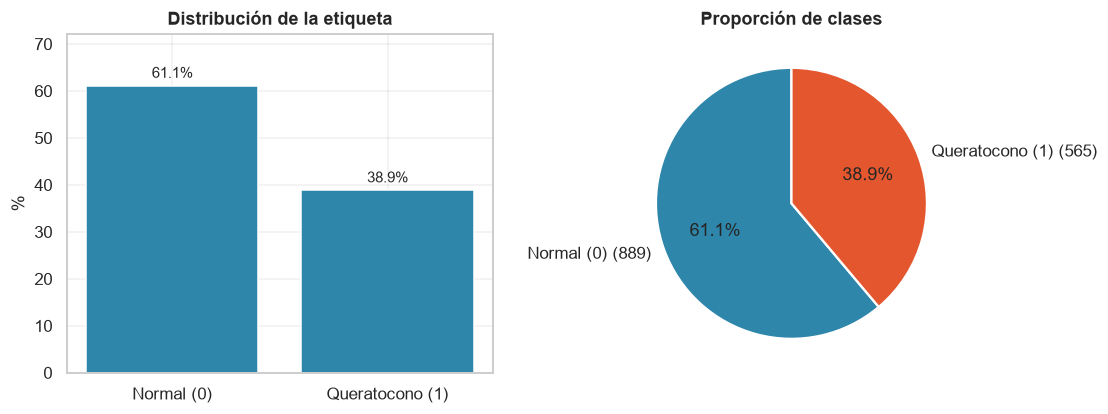
\includegraphics[width=0.85\linewidth]{img/eda/eda_clases.png}
                \caption{Distribución de los registros según la etiqueta diagnóstica.}
                \label{fig:eda_clases}
            \end{figure}

            La partición predefinida conserva esta proporción tanto en el conjunto de entrenamiento (61,13\,\% y 38,87\,\%) como en el de evaluación (61,17\,\% y 38,83\,\%), y los cinco \textit{folds} tienen un tamaño similar, de entre 230 y 236 registros cada uno.

            Dado que un mismo paciente puede aportar ambos ojos, se verificó que ningún paciente aparezca a la vez en el conjunto de entrenamiento y en el de evaluación. Esta condición se cumple, lo que evita una fuga de información, si los dos ojos de un paciente quedaran repartidos entre ambos conjuntos, el modelo sería evaluado sobre un paciente que ya ``conoció'' durante el entrenamiento, y su desempeño resultaría artificialmente alto. Además, la etiqueta es la misma para todos los registros de un paciente.

        \subsubsection*{Variables demográficas}

            El 65,13\,\% de los registros corresponde a mujeres y el 34,87\,\% a hombres, mientras que los ojos derecho e izquierdo están prácticamente balanceados (50,21\,\% y 49,79\,\%).

            La edad media es de 33,5 años en el grupo normal y de 27,9 años en el grupo con queratocono, cuyo registro más joven tiene 13 años (Figura~\ref{fig:eda_edad}). Este resultado es coherente con lo planteado en el Marco teórico respecto de la aparición temprana de la enfermedad~\cite{kcn_edad}, aunque describe a la muestra del \textit{dataset} y no a la población general.

            \begin{figure}[H]
                \centering
                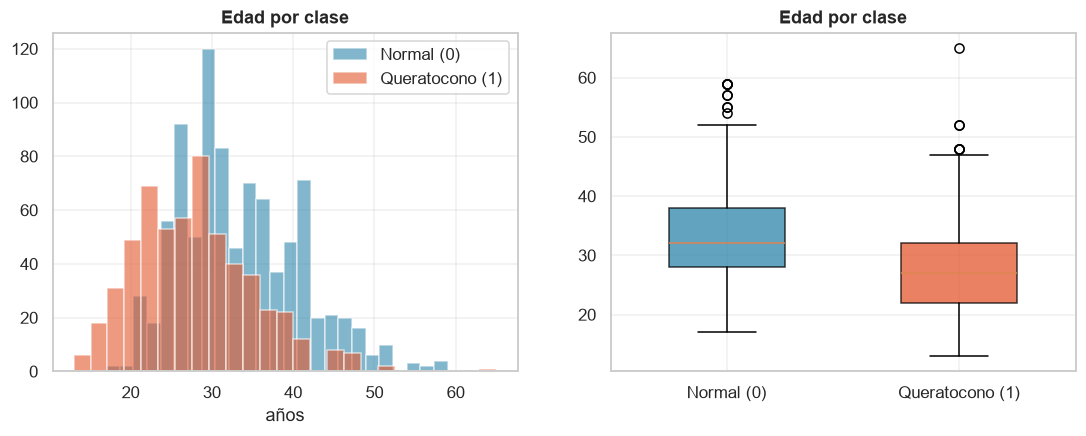
\includegraphics[width=0.85\linewidth]{img/eda/eda_edad.png}
                \caption{Distribución de la edad de los pacientes según la etiqueta diagnóstica.}
                \label{fig:eda_edad}
            \end{figure}

            En cuanto al sexo, al contar ojos, la proporción de queratocono resulta mayor en mujeres (40,76\,\%) que en hombres (35,31\,\%), con una diferencia estadísticamente significativa (prueba de chi-cuadrado, p\,=\,0,048). Sin embargo, al repetir el análisis contando pacientes, la diferencia se reduce (40,76\,\% frente a 38,81\,\%) y deja de ser relevante (p\,=\,0,658). El resultado inicial era, en parte, un efecto de contar los dos ojos de un mismo paciente como casos independientes. Se concluye que no hay evidencia de que un sexo tenga mayor probabilidad de queratocono en este \textit{dataset}. Aun así, como la muestra tiene mayoría de mujeres, conviene informar el desempeño del modelo por separado para cada sexo, para verificar que no favorezca a ninguno.

        \subsubsection*{Variables clínicas}

            La Figura~\ref{fig:eda_variables_clinicas} compara la distribución de cada variable clínica entre ambos grupos. En cada gráfico, la caja abarca la mitad central de los valores y la línea interior marca la mediana. Los ojos con queratocono presentan una curvatura máxima mayor (K max medio de 53,1 frente a 43,7 dioptrías), una córnea más delgada (espesor mínimo medio de 427,5 frente a 520,7~µm), mayor astigmatismo y una asfericidad más negativa, es decir, una córnea que se aparta más de la forma esférica. Estas diferencias coinciden con la descripción clínica de la enfermedad presentada en el Marco teórico.

            \begin{figure}[H]
                \centering
                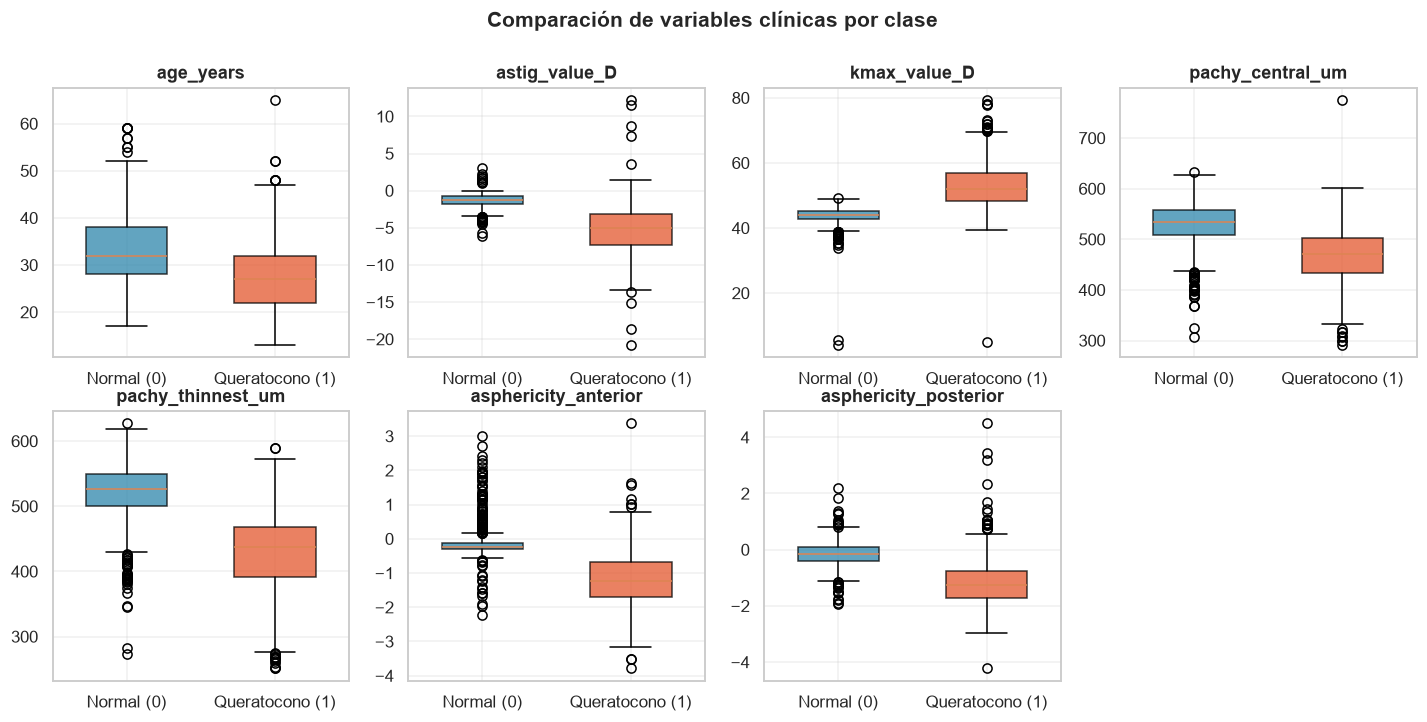
\includegraphics[width=\linewidth]{img/eda/eda_variables_clinicas.png}
                \caption{Comparación de las variables clínicas entre ojos normales y ojos con queratocono.}
                \label{fig:eda_variables_clinicas}
            \end{figure}

            Para cuantificar qué tanto se relaciona cada variable con el diagnóstico, se calculó su correlación con la etiqueta (Figura~\ref{fig:eda_correlacion}). La correlación toma valores entre \textminus{}1 y 1: cuanto más se aleja de cero, más se diferencia esa variable entre ojos normales y ojos con queratocono, y su signo indica si el valor aumenta o disminuye con la enfermedad. Las variables más relacionadas son el K max (0,69), el espesor mínimo (\textminus{}0,67), el astigmatismo (\textminus{}0,66) y la asfericidad anterior (\textminus{}0,64) y posterior (\textminus{}0,62), mientras que la ubicación del punto más delgado aporta poca información.

            \begin{figure}[H]
                \centering
                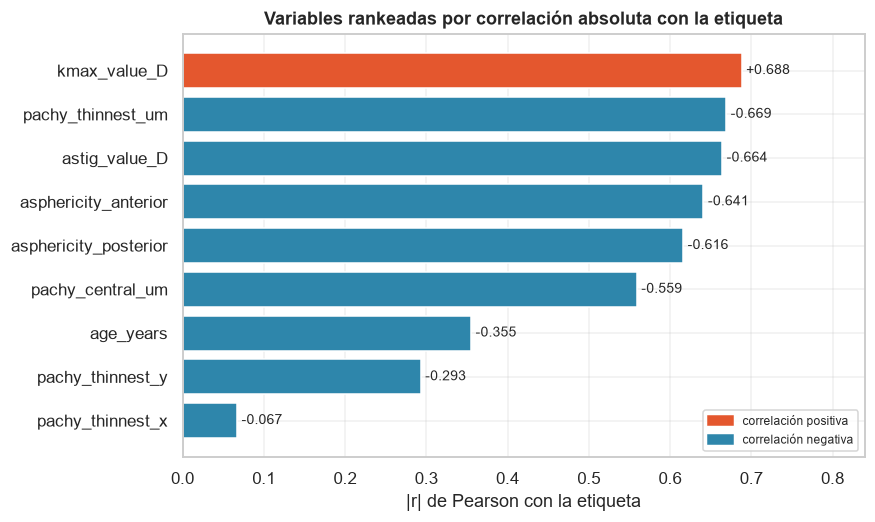
\includegraphics[width=0.68\linewidth]{img/eda/eda_correlacion.png}
                \caption{Variables clínicas ordenadas según su correlación con la etiqueta diagnóstica.}
                \label{fig:eda_correlacion}
            \end{figure}

            Muchas de estas variables también están relacionadas entre sí, ya que describen distintos aspectos de una misma deformación de la córnea. Esto debe tenerse en cuenta en el modelado para evitar que el modelo dependa de información redundante.

        \subsubsection*{Conclusiones del análisis}

            El análisis confirma que el \textit{dataset} es adecuado como punto de partida para el prototipo: tiene una partición bien construida, sin fugas de información entre pacientes, y sus variables clínicas muestran diferencias claras entre ojos normales y ojos con queratocono. Esto respalda la decisión de construir un modelo multimodal, en el que una rama analice estas variables junto a la rama que procesa los mapas corneales. Del análisis se desprenden las siguientes decisiones para la etapa de modelado:

            \begin{itemize}[leftmargin=*]
                \item Corregir el código de paciente \texttt{3E+132} y depurar los valores atípicos identificados antes del entrenamiento.

                \item Definir el tratamiento de las mediciones repetidas de un mismo ojo.

                \item Respetar la partición y los \textit{folds} predefinidos, de modo que los ojos de un mismo paciente queden siempre en el mismo conjunto.

                \item Evaluar el modelo priorizando la sensibilidad, en línea con el objetivo de reducir los falsos negativos, e informar su desempeño por separado para cada sexo.

                \item Transformar las variables de orientación (ejes en grados) antes de utilizarlas, ya que, por ejemplo, 1° y 179° representan orientaciones casi idénticas pese a la diferencia numérica.
            \end{itemize}
